% \iffalse meta-comment
%
% File: notebeamer.dtx
% -----------------------------------------------------------------------
%   Copyright (C) 2023-2025 by Mingyu Xia <myhsia@outlook.com>          *
%                                                                       *
%   This work may be distributed and/or modified under the conditions   *
%   of the LaTeX Project Public License (LPPL), either version 1.3c of  *
%   this license or (at your option) any later version.                 *
%   The latest version of this license is in                            *
%                                                                       *
%       http://www.latex-project.org/lppl.txt                           *
%                                                                       *
%   and version 1.3c or later is part of all distributions of LaTeX     *
%   version 2008 or later.                                              *
%                                                                       *
%   This work has the LPPL maintenance status `maintained'.             *
%                                                                       *
%   The Current Maintainer of this work is Mingyu Xia.                  *
%                                                                       *
%   This work consists of the files notebeamer.dtx,                     *
%                                   notebeamer.ins,                     *
%                 the derived files notebeamer.sty,                     *
%           the documentation files notebeamer.pdf,                     *
%                               and README.md.                          *
% -----------------------------------------------------------------------
%
%   Any modification of this file should ensure that the copyright and
%   license information is placed in the derived files.
%
% -----------------------------------------------------------------------
%
%<*internal>
\iffalse
%</internal>
%
%<*readme>
[![CTAN Version](https://img.shields.io/ctan/v/notebeamer)](https://ctan.org/pkg/notebeamer)
[![GitHub Release](https://img.shields.io/github/v/release/myhsia/notebeamer)](https://github.com/myhsia/notebeamer/releases/latest)
[![GitHub Last Commit](https://img.shields.io/github/last-commit/myhsia/notebeamer)](https://github.com/myhsia/notebeamer/commits)
[![Actions Status](https://github.com/myhsia/notebeamer/workflows/Automated%20testing/badge.svg)](https://github.com/myhsia/notebeamer/actions)
[![GitHub Repo stars](https://img.shields.io/github/stars/myhsia/notebeamer)](https://github.com/myhsia/notebeamer)

The `notebeamer` Package
========================

The `notebeamer` package provides a method for inputting slides on note
papers quickly.

Overview
--------

The package provides the `\includebeamer` macro

    \includebeamer [<keys>] {<filename>} [<keys>]

to set the format that how the slides is arranged on note papers.

See `notebeamer.pdf` for more. Happy TeXing!

Issues
------

The issue tracker for `notebeamer` is currently located
[on GitHub](https://github.com/myhsia/notebeamer/issues).

Build status
------------

This project uses [GitHub Actions](https://github.com/features/actions)
as a hosted continuous integration service. For each commit, the build status
is tested using the current release of TeX Live.

_Current build status:_ ![build status](https://github.com/myhsia/notebeamer/actions/workflows/main.yaml/badge.svg?branch=main)

Copyright and License
---------------------

Copyright (C) 2023-2025 by Mingyu Xia <myhsia@outlook.com>

This work may be distributed and/or modified under the conditions
of the LaTeX Project Public License (LPPL), either version 1.3c of
this license or (at your option) any later version.
The latest version of this license is in

    http://www.latex-project.org/lppl.txt

and version 1.3c or later is part of all distributions of LaTeX
version 2008 or later.

This work has the LPPL maintenance status `maintained'.

The Current Maintainer of this work is **Mingyu Xia**.
%</readme>
%
%<*internal>
\fi
%</internal>
%
%<*driver>
\documentclass{l3doc}
\usepackage[pass]{geometry}
\usepackage{notebeamer, pdfpages}
\usepackage[mono = false]{libertine}
\AddToHook{env/function/before}{\vspace*{-.7\baselineskip}}
\AddToHook{env/syntax/after}   {\par\vspace*{.2\baselineskip}}
\makeatletter
\def \@key  #1{\textcolor{red}{\textbf{\texttt{#1}}}\:\texttt{=}\:}
\def \s@key #1{\textcolor{red}{\texttt{\textup{\textbf{#1}}}}}
\DeclareDocumentCommand \key s {\IfBooleanTF{#1}\s@key\@key}
\DeclareCommandCopy \val \meta
\def \TFF {true\textup{\textbar\textbf{false}}}
\def \TTF {\textup{\textbf{true}\textbar}false}
\def \HoLogo@ApLaTeX #1{^^A
  \HOLOGO@mbox {A\kern -.05em p\kern -.05em \hologo{LaTeX}}}
\makeatother
\newlist{keyval}{itemize}{10}
\setlist[keyval]{leftmargin = 0pt, labelsep = 0pt}
\makeindex
\begin{document}
  \DocInput{\jobname.dtx}
\end{document}
%</driver>
% \fi
%
% \title{^^A
%   The \pkg{notebeamer} Package\thanks{^^A
%     \url{https://github.com/myhsia/notebeamer},
%     \url{https://ctan.org/pkg/notebeamer}^^A
%    }^^A
% }
%
% \author{^^A
%   Mingyu Xia \texttt{<^^A
%     \href{mailto:myhsia@outlook.com}{myhsia@outlook.com}^^A
%     \texorpdfstring{\:\textbar\:}{, }^^A\href{mailto:xiamingyu@westlake.edu.cn}
%     {xiamingyu@westlake.edu.cn}>^^A
%   }^^A
% }
%
% \date{Released 2025-07-21\quad \texttt{v4.4A}}
%
% \maketitle
%
% \begin{documentation}
%
% \section{Introduction}
%
% The \pkg{notebeamer} package provides an easy way to print slides on note
% pages quickly, developed by \pkg{expl3} based on \pkg{tikz}.
% It supports various compilation methods, such as
% \hologo{pdfLaTeX}, \hologo{XeLaTeX}, \hologo{ApLaTeX}, \hologo{LuaLaTeX}, etc.
%
% \section{Usage}
%
% To load this package, write the line
% \begin{quote}
%   |\usepackage{notebeamer}|
% \end{quote}
%
% \begin{function}{\includebeamer}
%   \begin{syntax}
%     \cs{includebeamer} \oarg{keyvals} \marg{filename} \oarg{keyvals}
%   \end{syntax}
%   The \cs{includebeamer} command can create pages with note lines, and import
%   the specific pages of the \file{.pdf} file on the left side of the note
%   pages. The mandatory argument can set the \file{.pdf} file that will be
%   inserted. The optional argument accepts the following keys
%   \begin{keyval}
%     \item [\key{color}] \val{str} can set the note lines' color
%     (Default: black), this key's name could be omitted.
%     \item [\key{ratio}] \val{fp num} can set imported slides' ratio and empty
%     area's width (Default: |0.5|).
%     \item [\key{sep}] \val{dim} can set the vertical space between slides
%     (Default: |2ex|).
%     \item [\key{nup}] \val{int} can set the number of slides on every page
%     (Default: |3|).
%     \item [\key{pages}] \val{comma-separated list} can select pages to insert.
%     The list could contain ranges of page numbers.
%     (Default: |1|).
%     \item [\key{lines}] \val{int} can set the number of lines on every page.
%     \item [\key{lineno}] \val{\TFF} can set whether to show the line numbers
%     (Default: |false|).
%     \item [\key{lhead, rhead}] \val{str} can set the left / right header of
%     the pages.
%   \end{keyval}
% \end{function}
% 
% \section{Working Example}
%
% Macros like \cs[no-index]{newgeometry}, and \cs[no-index]{pagecolor}, etc.,
% could be used for assistance.
%
% \verbatiminput{notebeamer-demo.tex}
% \noindent
% The effect of the above example is exhibited on the next page.
%
% 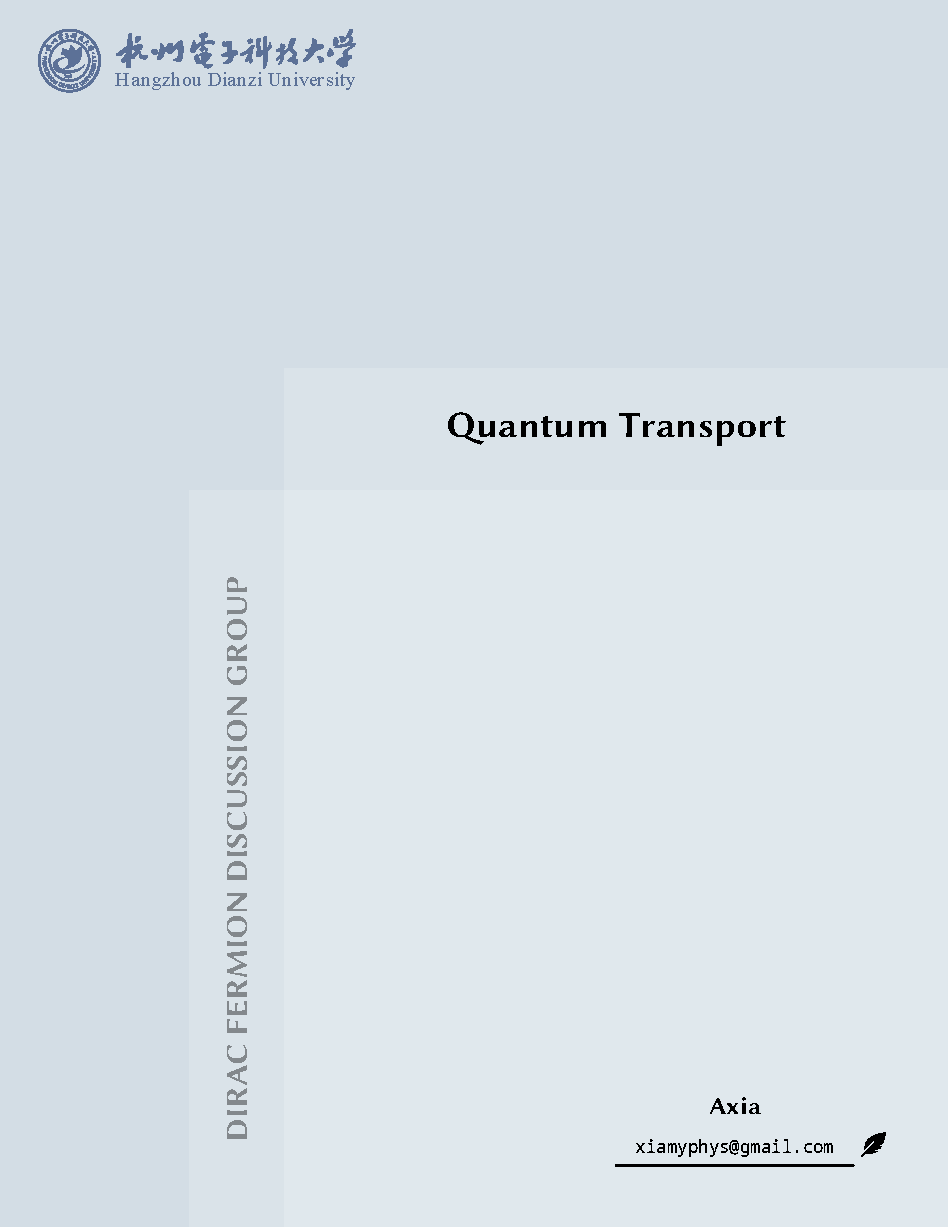
\includepdf[pages = -, nup = 2x2, frame]{notebeamer-demo.pdf}
% 
% \end{documentation}
%
% \begin{implementation}
%
% \section{The Source Code}
%
%    \begin{macrocode}
%<*package>
%    \end{macrocode}
%
%    \begin{macrocode}
%<@@=ntbm>
%    \end{macrocode}
%
%    \begin{macrocode}
\ProvidesExplPackage {notebeamer} {2025-07-21} {v4.4A}
  {Package for printing slides on note pages}
%    \end{macrocode}
%
%    \begin{macrocode}
\cs_if_exist:NF \graphics_include:nn
  { \RequirePackage{l3graphics} }
\RequirePackage{tikz, tikzpagenodes}
%    \end{macrocode}
%
% \subsection{User's Interface}
%
% \begin{macro}{\includebeamer}
%   Define the \cs{includebeamer} command.
%    \begin{macrocode}
\NewDocumentCommand \includebeamer { O{} m O{} }
  {
    \group_begin:
    \keys_set:nn { notebeamer / includebeamer } { #1, #3 }
    \@@_include_aux:n {#2}
    \group_end:
  }
%    \end{macrocode}
% \begin{variable}
%   {
%     \l_@@_include_color_tl , \l_@@_include_pages_tl  ,
%     \l_@@_include_nup_int  , \l_@@_include_lines_int ,
%     \l_@@_include_ratio_fp , \l_@@_include_sep_dim   ,
%     \l_@@_include_lhead_tl , \l_@@_include_rhead_tl
%   }
%   Key--value definitions for the \cs{includebeamer} command.
%    \begin{macrocode}
\keys_define:nn { notebeamer / includebeamer }
  {
    color   .tl_set:N   = \l_@@_include_color_tl,
      color .initial:n  = black,
    pages   .tl_set:N   = \l_@@_include_pages_tl,
      pages .initial:n  = 1,
    nup     .int_set:N  = \l_@@_include_nup_int,
      nup   .initial:n  = 3,
    lines   .int_set:N  = \l_@@_include_lines_int,
    lineno  .bool_set:N = \l_@@_include_lineno_bool,
      lineno .initial:n = false,
      lineno .default:n = true,
    ratio   .fp_set:N   = \l_@@_include_ratio_fp,
      ratio .initial:n  = .5,
    sep     .dim_set:N  = \l_@@_include_sep_dim,
      sep   .initial:n  = 2ex,
    lhead   .tl_set:N   = \l_@@_include_lhead_tl,
    rhead   .tl_set:N   = \l_@@_include_rhead_tl,
    unknown .code:n     = \tl_if_novalue:nF {#1}
      { \tl_set_eq:NN \l_@@_include_color_tl \l_keys_key_tl }
  }
%    \end{macrocode}
%   \end{variable}
% \end{macro}
%
% \subsection{Internal Auxiliary}
%
% \begin{variable}{\l_@@_nup_dim, \l_@@_include_ratio_dim}
%   Store the heights and widths of the logical pages in a specific nup.
%    \begin{macrocode}
\dim_new:N \l_@@_nup_dim
\dim_new:N \l_@@_include_ratio_dim
%    \end{macrocode}
% \end{variable}
% \newpage
% \begin{variable}{\l_@@_pages_total_int, \l_@@_pages_residue_int}
%   Store the number of total physical pages and residue logical pages.
%    \begin{macrocode}
\int_new:N \l_@@_pages_total_int
\int_new:N \l_@@_pages_residue_int
%    \end{macrocode}
% \end{variable}
%
% \begin{variable}{\l_@@_tmpa_clist}
%   Store the results of \cs{@@_range_to_list:nN}.
%    \begin{macrocode}
\clist_new:N \l_@@_tmpa_clist
%    \end{macrocode}
% \end{variable}
%
% \begin{macro}{\@@_include_aux:n}
%   Define the auxiliary command for \cs{includebeamer}.
%    \begin{macrocode}
\cs_new_protected_nopar:Npn \@@_include_aux:n #1
  {
    \graphics_get_pagecount:nN {#1} \l_@@_include_filepages_int
    \dim_set:Nn \l_@@_nup_dim { \textheight/\l_@@_include_nup_int }
    \dim_set:Nn \l_@@_include_ratio_dim
      { \fp_use:N \l_@@_include_ratio_fp \textwidth }
    \tl_if_eq:NnTF \l_@@_include_pages_tl { - }
      {
        \@@_range_to_list:nN
          { 1 - \l_@@_include_filepages_int } \l_@@_tmpa_clist
      }
      {
        \exp_args:NV \@@_range_to_list:nN
          { \l_@@_include_pages_tl } \l_@@_tmpa_clist
      }
    \int_set:Nn \l_@@_pages_total_int
      {
        \fp_eval:n
          { ceil
              ( \clist_count:N \l_@@_tmpa_clist/
                  \l_@@_include_nup_int, 0
              ) - 1
          }
      }
    \int_set:Nn \l_@@_pages_residue_int
      {
        \int_eval:n
          {
            \clist_count:N \l_@@_tmpa_clist -
            \l_@@_include_nup_int * \l_@@_pages_total_int
          }
      }
    \int_step_inline:nn { \int_use:N \l_@@_pages_total_int }
      {
        \clearpage
        \@@_empty_note_aux:
        \int_step_inline:nn { \l_@@_include_nup_int }
          {
            \tikz [ remember~picture, overlay ]
              \node [ xshift = \l_@@_include_ratio_dim/2,
                      yshift = \fp_eval:n { -####1 + .5 } \l_@@_nup_dim
                    ] at (current~page~text~area.north~west)
                {
                  \includegraphics
                    [ height = \dim_eval:n
                        { \l_@@_nup_dim - \l_@@_include_sep_dim },
                      page = \clist_item:Nn \l_@@_tmpa_clist
                        { ####1 + \l_@@_include_nup_int * ( ##1 - 1 ) }
                    ] {#1}
                };
          }
        \clearpage
      }
    \@@_empty_note_aux:
    \int_step_inline:nn { \int_use:N \l_@@_pages_residue_int }
      {
        \tikz [ remember~picture, overlay ]
          \node [ xshift = \l_@@_include_ratio_dim/2,
                  yshift = \fp_eval:n {( -##1 + .5 )} \l_@@_nup_dim
                ] at (current~page~text~area.north~west)
            {
              \includegraphics
                [ height = \dim_eval:n
                    { \l_@@_nup_dim - \l_@@_include_sep_dim },
                  page = \clist_item:Nn \l_@@_tmpa_clist
                    {
                      \l_@@_include_nup_int *
                      \l_@@_pages_total_int + ##1
                    }
                ] {#1}
            };
      }
    \clearpage
  }
%    \end{macrocode}
% \end{macro}
%
% \begin{macro}{\@@_empty_note_aux:}
%   Define the auxiliary command for creating empty note line page.
%    \begin{macrocode}
\cs_new_protected_nopar:Nn \@@_empty_note_aux:
  {
    \begin { tikzpicture } [ remember~picture, overlay ]
      \draw [ very~thick, \l_@@_include_color_tl, opacity = .8 ]
        (current~page~text~area.north~west) --
        (current~page~text~area.north~east)
       node [ at~start, above~right, font = \Large \bfseries ]
        { \l_@@_include_lhead_tl }
       node [ above~left, font = \Large \bfseries ]
        { \l_@@_include_rhead_tl };
      \draw [ very~thick, \l_@@_include_color_tl, opacity = .8 ]
        (current~page~text~area.south~west) --
        (current~page~text~area.south~east);
      \int_step_inline:nn { \l_@@_include_lines_int - 1 }
        {
          \draw [ thick, \l_@@_include_color_tl, opacity = .6 ]
            ([xshift = \l_@@_include_ratio_dim,
              yshift = -\textheight/\l_@@_include_lines_int * ##1
             ]current~page~text~area.north~west) --++
            (\dim_eval:n { \textwidth - \l_@@_include_ratio_dim },0);
          \bool_if:nT \l_@@_include_lineno_bool
            {
              \node [ font = \footnotesize, \l_@@_include_color_tl,
                      opacity = .4, right ] at
                ([xshift = \textwidth,
                  yshift = -\textheight/\l_@@_include_lines_int * (##1 - .5)
                 ]current~page~text~area.north~west)
                { \int_eval:n { ##1 } };
            }
        }
      \node [ font = \footnotesize, \l_@@_include_color_tl,
              opacity = .4, right ] at
        ([xshift = \textwidth,
          yshift = -\textheight + \textheight/\l_@@_include_lines_int * .5
         ]current~page~text~area.north~west)
        { \int_eval:n { \l_@@_include_lines_int } };
    \end { tikzpicture }
    \pagestyle { empty }
  }
%    \end{macrocode}
% \end{macro}
%
% \begin{variable}{\l_@@_tmpa_seq, \l_@@_tmpb_seq}
%   Store the results of 2D array segmentation.
%    \begin{macrocode}
\seq_new:N \l_@@_tmpa_seq
\seq_new:N \l_@@_tmpb_seq
%    \end{macrocode}
% \end{variable}
%
% \begin{macro}{\@@_range_to_list:nN}
%   Convert the combination of number and number range to a list.
%    \begin{macrocode}
\cs_new_protected_nopar:Npn \@@_range_to_list:nN #1#2
  {
    \clist_clear:N #2
    \seq_set_split:Nnn \l_@@_tmpa_seq { , } {#1}
    \seq_map_inline:Nn \l_@@_tmpa_seq
      {
        \tl_if_in:nnTF {##1} { - }
          {
            \seq_set_split:Nnn \l_@@_tmpb_seq { - } {##1}
            \int_step_inline:nnn
              { \seq_item:Nn \l_@@_tmpb_seq { 1 } }
              { \seq_item:Nn \l_@@_tmpb_seq { 2 } }
              { \clist_put_right:Nn #2 {####1} }
          } { \clist_put_right:Nn #2 {##1} }
      }
  }
%    \end{macrocode}
% \end{macro}
%
%    \begin{macrocode}
%</package>
%    \end{macrocode}
%
% \end{implementation}
%
% \PrintIndex
